\def\micro{\mu m}
\def\um{$\micro$ }
\def\degreesC{$\degree C$ }
\def\percent{$\%$ }
\documentclass[10pt,a4paper,oneside]{article}
\usepackage[left=2cm,right=2cm,top=2cm,bottom=2cm]{geometry}

\usepackage[dvipsnames]{xcolor}

%%  -------------------------------------------------------------------
%%      GDS II layer, regarding MOSIS SCMOS layer map
%%  -------------------------------------------------------------------
% GDS II #41 - P_WELL
\definecolor{pwell}{rgb}{1.0, 0.74, 0.53}   % macaroni and cheese
% GDS II #42 - N_WELL
\definecolor{nwell}{rgb}{0.61, 0.87, 1.0}  % columbia blue
\definecolor{pbase}{rgb}{1.0, 0.51, 0.26}  % mango tango
\definecolor{nbase}{rgb}{0.0, 0.75, 1.0}   % capri 
% GDS II #43 - ACITVE
\definecolor{active}{rgb}{0.9, 0.4, 0.38}   % light carmine pink
% GDS II #45 - N_PLUS_SELECT
\definecolor{nimplant}{rgb}{0.45, 0.76, 0.983}% maya blue
% GDS II #44 - P_PLUS_SELECT
\definecolor{pimplant}{rgb}{1.0, 0.51, 0.26}% mango tango
% GDS II #46 - POLY
\definecolor{poly}{rgb}{0.56, 0.93, 0.56}   % light green
% GDS II #25 - CONTACT
\definecolor{contact}{rgb}{0.83, 0.83, 0.83}% light gray
% GDS II #49 - METAL1
\definecolor{metal1}{rgb}{0.38, 0.31, 0.86} % majorelle blue
% GDS II #50 - VIA1
\definecolor{via1}{rgb}{0.83, 0.83, 0.83}   % light gray
% GDS II #51 - METAL2
\definecolor{metal2}{rgb}{0.04, 0.85, 0.32} % malachite
% GDS II #61 - VIA2
\definecolor{via2}{rgb}{0.83, 0.83, 0.83}   % light gray
% GDS II #63 - METAL3
\definecolor{metal3}{rgb}{0.98, 0.93, 0.37} % maize
% GDS II #30 - VIA3
\definecolor{via3}{rgb}{0.83, 0.83, 0.83}   % light gray
% GDS II #31 - METAL4
\definecolor{metal4}{rgb}{0.75, 0.25, 0.0}  % mahogany
% GDS II #32 - VIA4
\definecolor{via4}{rgb}{0.83, 0.83, 0.83}   % light gray
% GDS II #33 - METAL5
\definecolor{metal5}{rgb}{0.79, 0.08, 0.48} % magenta (dye)
% GDS II #36 - VIA5
\definecolor{via5}{rgb}{0.83, 0.83, 0.83}   % light gray
% GDS II #37 - METAL6
\definecolor{metal6}{rgb}{0.11, 0.35, 0.02} % lincoln green
% GDS II #29 - SILICIDE_BLOCK
\definecolor{silicide-block}{rgb}{0.98, 0.94, 0.9}  % linen
% GDS II #52 - GLASS
\definecolor{glass}{rgb}{1.0, 1.0, 0.88}    % light yellow
% GDS II #26 - PADS
\definecolor{pads}{rgb}{0.75, 1.0, 0.0}     % lime (color wheel)

\definecolor{resist}{rgb}{0.71, 0.4, 0.11}  % light brown

\definecolor{silicide}{rgb}{0.29, 0.33, 0.13}
\definecolor{titanium}{rgb}{0.8, 0.58, 0.46}

\def\OpacityLayout {0.5}

%
% physical
%
\definecolor{substrate}{rgb}{0.96, 0.94, 0.93}  % isabelline
\definecolor{nitride}{rgb}{1.0, 0.03, 0.0}
\definecolor{gateoxide}{rgb}{0.88, 1.0, 1.0}    % light cyan
\definecolor{isolationoxide}{rgb}{0.84, 0.79, 0.87}% languid lavender

\usepackage[utf8]{inputenc}
\usepackage[english]{babel}
\usepackage{forloop}
\usepackage{amsmath}
\usepackage{amsfonts}
\usepackage{amssymb}
\usepackage{gensymb}
\usepackage{mdframed}
\usepackage{graphicx}
\usepackage{tikz}
\usetikzlibrary{arrows,automata,shapes}
\usepackage[siunitx]{circuitikz}
\usepackage{makecell}
\usepackage{array}

\def\WaferClean{
\begin{tikzpicture}\node [fill=cyan, rounded corners=5pt] {\large Clean};\end{tikzpicture}}
\def\WaferSemiClean{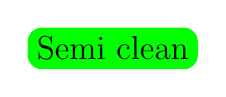
\begin{tikzpicture}\node [fill=green, rounded corners=5pt] {\large Semi clean};\end{tikzpicture}}
\def\WaferNonStandard{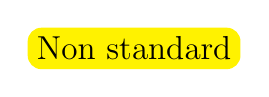
\begin{tikzpicture}\node [fill=yellow, rounded corners=5pt] {\large Non standard};\end{tikzpicture}}

\usepackage[colorlinks=true,linkcolor=blue,urlcolor=black,bookmarksopen=true]{hyperref}
\usepackage{bookmark}
\usepackage{hyperref}
\usepackage{sepfootnotes}
\usepackage{lipsum,tocloft} 
\usetikzlibrary{positioning}
\usetikzlibrary{patterns}

\usepackage{float}
\floatstyle{boxed} 
\restylefloat{figure}

\title{Physics essentials for LibreSilicon}
\date{\today}
\author{David Lanzendörfer}
\makeindex

\newcounter{ct}
\def\CrossSectionOnly{0.3}
\def\CrossAndTopSection{0.2}
\def\CrossAndTopSectionBig{0.3}
\def\VLSILayout{0.4}

\DeclareMathOperator\erfc{erfc}

\setlength{\parindent}{0pt} % get rid of annoying indents

\begin{document}
\begin{abstract}
	Copyright © 2017 LANCEVILLE TECHNOLOGY GROUP CO., LIMITED. All rights reserved. \\

This process is licensed under the Libre Silicon public license; you can redistribute it and/or modify it under the terms of the Libre Silicon public license
as published by the Libre Silicon alliance, either version 1 of the License, or (at your option) any later version.

This design is distributed in the hope that it will be useful, but WITHOUT ANY WARRANTY; without even the implied warranty of MERCHANTABILITY or FITNESS FOR A PARTICULAR PURPOSE.
See the Libre Silicon Public License for more details. \\

This document is part of the specification of the free silicon manufacturing standard for manufacturing the LibreSilicon standard logic cells\footnote{\url{https://github.com/chipforge/StdCellLib}} and related free technology nodes from the LibreSilicon project.

For this initial revision 0.1 a gate-first approach has been chosen which led to the choice of polysilicon as the gate electrode material because of the simplicity of the gate alignment.
For better isolation properties of the transistors and gates in overall a box-isolation approach has been chosen.
All of these choices have been made with the future scale down from the recent $1 \mu m$ to smaller structure sizes.
\textbf{This process is for manufacturing $1 \mu m$ only!}
But further releases which will have been tested with smaller structure sizes can be expected.

\end{abstract}

\newpage
\tableofcontents

\maketitle
In this document we deal with all the physics related to solid state device manufacturing.
In case there is anything unclear, please look up this document and its chapters.
\section{Getting doping from resistance}
In many cases the supplier will only provide the resistance per length specification for their substrate and won't give you the dopant concentration numbers.
In this case you will have to find these numbers out yourself by converting it from the numbers they've provided.

\begin{figure}[H]
	\centering
	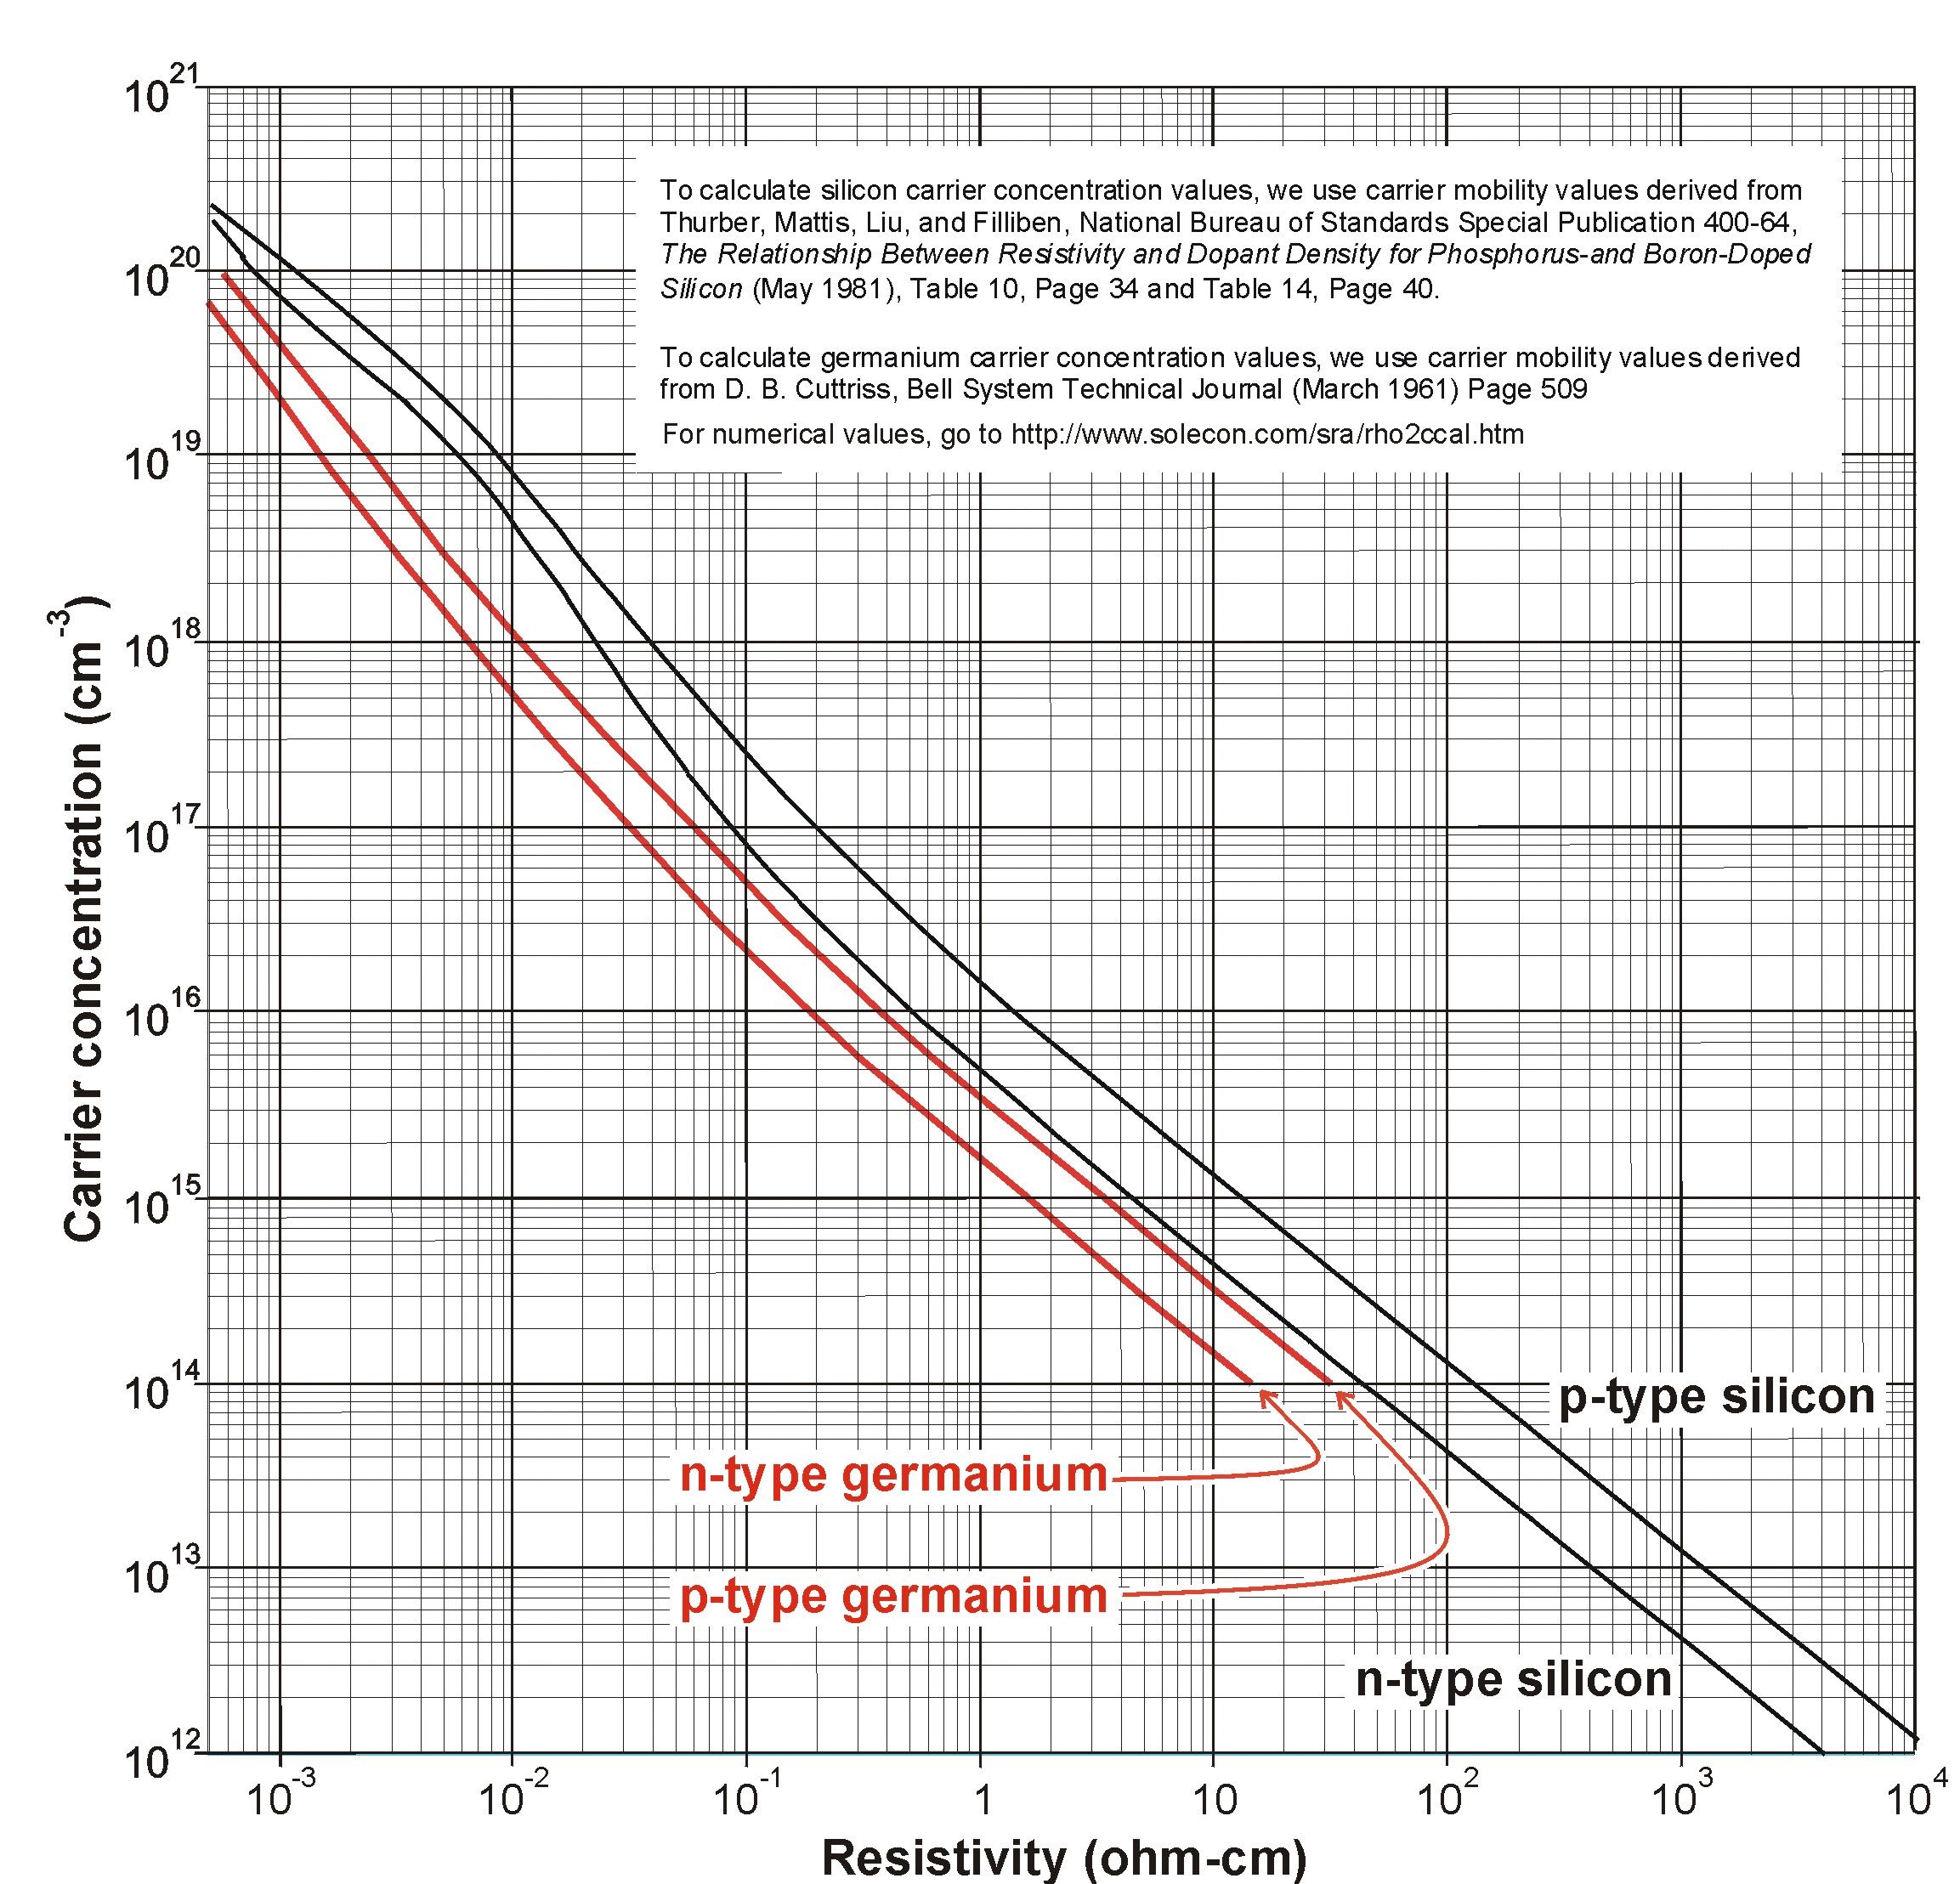
\includegraphics[width=0.5\textwidth]{resistance_doping.png}
	\caption{R-L-dopant relation}
	\label{r_l_nd_relation}
\end{figure}

You can either use the graphics from \autoref{r_l_nd_relation} and determine the dopant concentration graphically, which is very very imprecise or use a online tool like the one from Solecon\footnote{\url{http://www.solecon.com/sra/rho2ccal.htm}}

Germanium is being included in this graphics just in case someone is going to fork this process based on Germanium substrate.
\newpage
\subsection{Infusion}
The redistribution process depends on the ratio of the solubility of the doping material in silicon and SiO$ _2$. At the Si/SiO$ _2$ interface the dopants are redistributed by segregation until the ratio of their concentration at the interface is the same as the ratio of their solubility in both materials. The ratio of dopant solubility is expressed by the segregation coefficient $m$ which is

\begin{equation}
\displaystyle m = \frac{
	\mathrm{solubility\ in\ silicon}
	}{
	\mathrm{solubility\ in\ SiO_2}
	}
\end{equation}

As listed in \autoref{table_diffusion_coeff} below there are dopant species which solubilize better in SiO$ _2$ than in silicon ($ m < 1$) and species which have a reversed behavior ($ m > 1$).
In case of $ m < 1$, as for Boron, the dopant concentration is enhanced at the SiO$ _2$ side, whereas beneath the interface, there is a dopant depletion at the silicon surface.
For reversed solubility ratios ($ m > 1$, like Phosphorus), only few dopant atoms penetrate the interface.
In order to obtain the by $ m$ determined concentration ratio at the interface, dopant atoms from deeper silicon zones diffuse back to the surface zone.
Therefore, the dopant concentration at the silicon surface is enhanced, as illustrated in \autoref{graph_figure}b.
In \autoref{graph_figure} $ C_c$ denotes the dopant concentration in the silicon surface zone before oxidation. $ x$ is the distance from the silicon surface.

\begin{figure}[H]
	\centering
	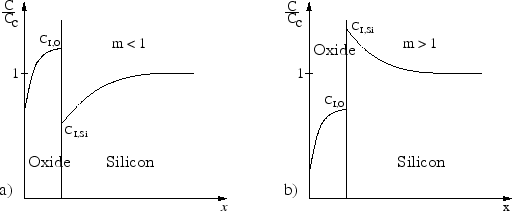
\includegraphics[width=0.75\linewidth]{img349.png}
	\caption{Schematic illustration of dopant redistribution}
	\label{graph_figure}
\end{figure}
\begin{table}[H]
	\centering
	\begin{tabular}{|c|c|c|c|c|c|}
		\hline
		Dopant species &
		Boron &
		Phosphor &
		Antimon &
		Arsen &
		Gallium \\
		\hline
		$m$ &
		0.1-0.3 &
		10 &
		10 &
		10 &
		20 \\
		\hline
	\end{tabular}
	\caption{Segregation coefficients $m$ for important dopant species in silicon}
	\label{table_diffusion_coeff}
\end{table}
\newpage
\subsection{Constant source diffusion (Predeposition)}

Although the diffusion process of donors and acceptors into the silicon crystal is a three dimensional process for simplicity we first only discuss the one dimensional mathematics for it in order to get a "simple" equation for the depth-time-temperature relation.

\begin{mdframed}[linewidth=2pt,linecolor=red]
This is only valid for a constant source of dopants on the surface of the wafer (for instance gas).
These equations are being used for predicting the pre-deposition step (in case this process would be adapted by someone for predeposition instead of ion implant)
\end{mdframed}

We start with Ficks law (for all German speakers: Yes that's his name, not me shouting about this problem) where the dopant concentration N is coupled with time and place
\begin{equation}
\frac{\partial N}{\partial t} = D \cdot \frac{\partial^2 N}{\partial x^2}
\end{equation}

The diffusion coefficient is as well material as well as temperature dependent  and can be calculated with the following equation:
\begin{equation}
D = D_0 \cdot \exp\left(-\frac{E_a}{k \cdot T}\right)
\end{equation}
With $k=8.62 \cdot 10^{-5} \frac{eV}{K}$ being the Boltzman constant and in \autoref{absolute_diffusion_coefficients} we can see the $D_0$ and $E_a$ values for the most common materials\footnote{ISBN 3-8023-1588:Hoppe Bernhard, Mikroelektronik 2, Page 24, Table 2.1} which we can use within the further calculations for our well dimensioning phases. The temperature usually is in the area of $1000\degree C$ or in Kelvin $1273.15\degree K$.
\begin{table}[H]
	\centering
	\begin{tabular}{|c|c|c|}
		\hline
		Element &
		$D_0$ $\left[\frac{cm^2}{s}\right]$ &
		$E_a$ $\left[eV\right]$ \\
		\hline
		P &
		10.50 &
		3.69 \\
		\hline
		As &
		0.32 &
		3.56 \\
		\hline
		Sb &
		5.60 &
		3.95 \\
		\hline
		B &
		10.50 &
		3.69 \\
		\hline
		Al &
		8.00 &
		3.47 \\
		\hline
		Ga &
		3.60 &
		3.51 \\
		\hline
		Cu &
		0.0025 &
		0.65 \\
		\hline
	\end{tabular}
	\label{absolute_diffusion_coefficients}
	\caption{$D_0$ and $E_a$ values for Boron and Phosphorus}
\end{table}

The law stated above
\begin{equation}
\frac{\partial N}{\partial t} = D \cdot \frac{\partial^2 N}{\partial x^2} 
\end{equation}
has the same form as the temperature conductivity equation (Laplace) for which we already have a general solution
\begin{equation}
\frac{\partial u}{\partial t} = a^2 \cdot \frac{\partial^2 u}{\partial x^2} 
\end{equation}

Which means that we can map the general solution for the temperature conductivity equations after Laplace
\begin{equation}
u(x,t) = \frac{1}{2 \cdot a \cdot \sqrt{\pi \cdot t}} \cdot \int_{-\infty}^{\infty}{f(a)\cdot\exp\left(\frac{-(x-a)^2}{4 \cdot a^2 \cdot t^2}\right)}da
\end{equation}
to our Ficks law with $a=\sqrt{D}$ und $u=N$
\begin{equation}
N(x,t) = \frac{1}{2 \cdot \sqrt{D} \cdot \sqrt{\pi \cdot t}} \cdot \int_{-\infty}^{\infty}{f(\sqrt{D})\cdot\exp\left(\frac{-(x-\sqrt{D})^2}{4 \cdot D \cdot t^2}\right)}da
\end{equation}
with the edge conditions
\begin{equation}
N( x=0 , t > 0 ) = N_0
\end{equation}
\begin{equation}
N( x \geq 0 ,  t = 0 ) = 0
\end{equation}
we get the resulting function from the solving process for the Laplace temperature conduction equations
\begin{equation}
u(x,t)=u_0 \cdot erfc\left(\frac{x}{2 \cdot a \cdot \sqrt{t}}\right)
\end{equation}
with the error function being an integral of the form
\begin{equation}
erfc(z)
=
\left(1-\frac{2}{\sqrt{\pi}}\right)\cdot\int_0^z{e^{-a^2}}da
\end{equation}

Or in case of our dopant concentration equation we can replace a with the square root of the diffusion coefficient in order to get the error function for our dopant density euqtion:
\begin{equation}
erfc(z)
=
\left(1-\frac{2}{\sqrt{\pi}}\right)\cdot\int_0^z{e^{-D}}d\sqrt{D}
\end{equation}
\begin{equation}
N(x,t)
=
N_0 \cdot erfc\left(\frac{x}{2 \cdot \sqrt{D \cdot t}}\right)
=
N_0 \cdot erfc\left(\frac{x}{x_l(t)}\right)
\end{equation}
Now we can extract the layer thickness respectively the depth of the well in dependency of the time and the temperature:
\begin{equation}
x_l(t) = 2 \cdot \sqrt{D \cdot t}
\end{equation}
\begin{equation}
x_l(t) = 2 \cdot \sqrt{D_0 \cdot \exp\left(-\frac{E_a}{k \cdot T}\right) \cdot t}
\end{equation}

And plot the result for multiple different drive in times
\begin{figure}[H]
	\centering
	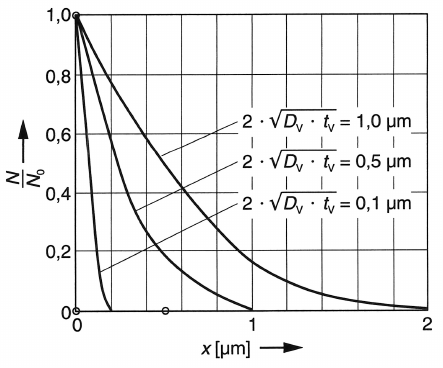
\includegraphics[scale=0.5]{dopants_depth.png}
	\caption{Different predeposition times}
\end{figure}

We can now describe the dosage based on the time and temperature of the diffusion

\begin{equation}
Q=\frac{2}{\sqrt{\pi}} \cdot N_0 \cdot \sqrt{D \cdot t}
\end{equation}

Where $N_0$ (concentration at the surface) equals the maximum solubility of a given element (e.g. Boron) within the given medium (e.g. Silicon).

\newpage
\subsection{Ion implant}
We can use the following equation to calculate the carrier distribution after implantation:
\begin{equation}
N(x,t)
=
N_p \exp\left(-\frac{(x-R_p)^2}{2\Delta R_p^2}\right)
=
\frac{Q}{\sqrt{2\pi}\Delta R_p}\exp\left(-\frac{(x-R_p)^2}{2\Delta R_p^2}\right)
\end{equation}

Where the projected range ($R_p$) and the projected straggle ($\Delta R_p$) need to be looked up in tables or looked up using an online tool like the one linked in the footnote\footnote{\url{http://cleanroom.byu.edu/rangestraggle}}
\subsection{Diffusion (Drive-in)}

\subsection{Vertical diffusion and junction formation (Well formation)}\label{building_wells}
The goal of most diffusions is to form pn junctions by converting p-type material to n-type material or vice versa.
In \autoref{junction_formation_plot}, for example, the wafer is uniformly doped n-type material with a concentration indicated by $N_B$, and the diffusing impurity is boron.
The point at which the diffused impurity profile intersects the background concentration is the mettalurgical junction depth ($x_j$).
The net impurity concentration at $x_j$ is zero.
Setting $N(x)$ equal to the background concentration $N_B$ at $x=x_j$ yields\footnote{Gerold W. Neudeck and Robert F. Pierret, Modular series on solid state devices, Volume V, Chapter 4}
\begin{equation}
x_j
=
2 \cdot\sqrt{D \cdot t \cdot \ln\left(\frac{N_0}{N_B}\right)}
\end{equation}
and
\begin{equation}
x_j
=
2 \cdot\sqrt{D \cdot t}
\cdot
\erfc^{-1}\left(\frac{N_B}{N_0}\right)
\end{equation}

for the Gaussian and complementary error function distributions, respectively.

In \autoref{junction_formation_plot}, the boron concentration $N$ exceeds $N_B$ to the left of the junction, and this region is p-type.
To the right of $x_j$, $N$ is less than $N_B$, and this region remains n-type.

To calculate the junction depth, we must know the background concentration $N_B$ of the original wafer.
Look at \autoref{r_l_nd_relation} for this purpose.

\begin{figure}[H]
	\centering
	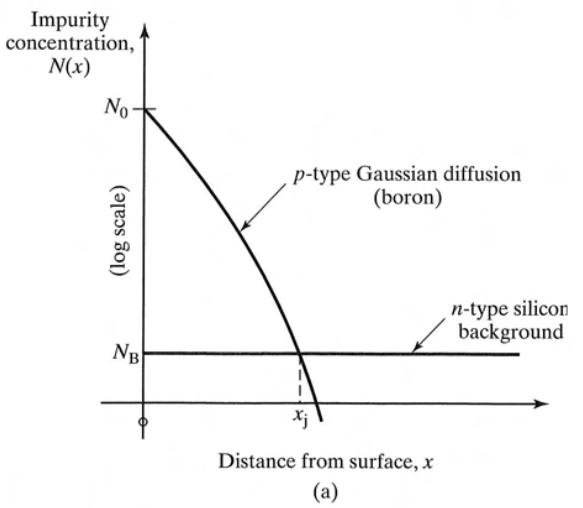
\includegraphics[scale=0.5]{well_formation1.png}
	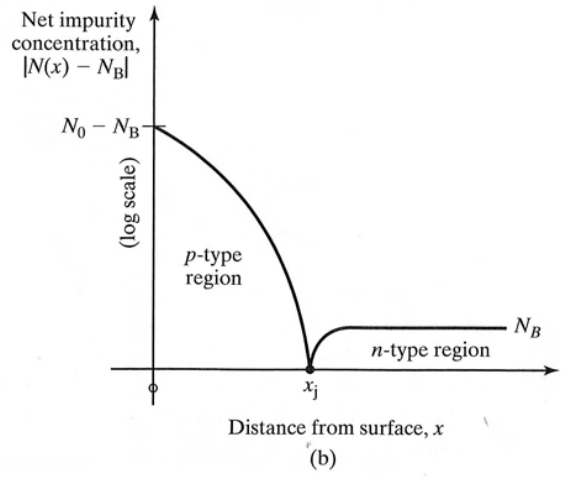
\includegraphics[scale=0.5]{well_formation2.png}
	\caption{Formation of a pn junction by diffusion: (a) An example of a p-type Gaussian diffusion into a uniformly doped n-type wafer; (b) net impurity concentration in the wafer.}
	\label{junction_formation_plot}
\end{figure}


\newpage
\section{MOS Capacitance}
\url{https://ecee.colorado.edu/~bart/book/book/chapter6/ch6_3.htm}

\newpage
\section{Threshold voltages ($V_T$)}

The threshold voltage dependence on the doping density is illustrated with \autoref{img:overview_doping_threshold} for both n-type and p-type MOSFETs with an aluminum gate metal.
\begin{figure}[H]
	\centering
	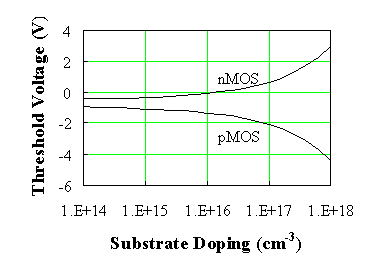
\includegraphics[scale=0.5]{doping_thresholds_overview.png}
	\caption{Threshold voltage of n-type (upper curve) and p-type (lower curve) MOSFETs versus substrate doping density.}
	\label{img:overview_doping_threshold}
\end{figure}
\begin{mdframed}[linewidth=2pt,linecolor=red]
We can directly switch $\frac{J}{C}$ with Volts because these two units are equal!\footnote{\url{https://en.wikipedia.org/wiki/Volt}}
Also $V_{th}$ will be treated as a constant for any further calculations within this document.\\

The same goes for the $eV$ to $V$ conversion, wherever we have work functions to potentials because (e.g. $\Phi_M$ for Aluminum):
$4.1 eV \approx 6.56892414528 10^{-19}J$ \\
$\Phi_M=\frac{E_M}{q}=\frac{4.1 eV}{q}=\frac{6.56892414528 10^{-19} J}{q} = \frac{6.56892414528 10^{-19} J}{1.602176634 10^{-19} C} \approx 4.099999966220953 \frac{J}{C} = \underline{4.1V}$ \\
\end{mdframed}

The formula for calculating the threshold voltage of a MOS device is the following:
\begin{equation}
V_T = V_{t-mos} + V_{FB}
\end{equation}
where $V_{t-mos}$ is the threshold voltage of an ideal MOS capacitor, $V_{FB}$ is the flat-band voltage and $V_{t-mos}$ is the threshold.
The MOS threshold voltage, $V_{t-mos}$ is calculated by considering the MOS capacitor structure that form the gate of the MOS transistor.

The ideal threshold voltage may be expressed as:
\begin{equation}
V_{t-mos}=2 \phi_F + \frac{Q_b}{C_{ox}}
\end{equation}
\begin{equation}
Q_b
=
\sqrt{2 \epsilon_{Si} \cdot q \cdot N  \cdot  ( \left| 2 \phi_F \right| + V_{SB}) }
\end{equation}
where $C_{ox}$ is the oxide capacitance and $Q_b$ which is called the bulk charge term.\\

The bulk potential is given for P substrate ($V_{Tp}$)
\begin{equation}
\phi_{Fp}
=
V_{th} \cdot ln\left(\frac{N_p}{N_i}\right)
\end{equation}
and N substrate  ($V_{Tn}$), respectively:
\begin{equation}
\phi_{Fn}
=
V_{th} \cdot ln\left(\frac{N_i}{N_n}\right)
\end{equation}

$V_{th}$ is the thermal voltage.\footnote{\url{https://en.wikipedia.org/wiki/Boltzmann_constant\#Role_in_semiconductor_physics:_the_thermal_voltage}}
\begin{equation}
V_{th} = \frac{k T}{q} \approx 0.026 \frac{J}{C} = 0.026 V = 26mV
\end{equation}

Since we connect bulk and source $V_{SB}=0$ we can simplify the equation to become
\begin{equation}
Q_b
=
\sqrt{2\cdot\epsilon_{Si}\cdot q\cdot N \cdot  ( \left| 2 \cdot \phi_F \right|) }
\end{equation}
\begin{equation}
Q_b
=
2\cdot\sqrt{\epsilon_{Si}\cdot q\cdot N \cdot \left| \phi_F \right| }
\end{equation}


$V_{FB}$, is given by:
\begin{equation}
V_{FB}
=
\phi_{MS}-\frac{Q_{SS}}{C_{ox}}-\frac{1}{C_{ox}}\int_{0}^{t_{ox}}\frac{x}{x_{ox}}\rho(x) dx
\end{equation}

Because we're not yet dealing with non-volatile memory devices which contain an oxide surface state charge we can just $\rho(x)=0$.
$Q_{SS}$ is a value which has to be measured.

\begin{equation}
V_{FB}
=
\phi_{MS} - \frac{Q_{SS}}{C_{ox}}
\end{equation}

This brings us to a general equation for the threshold voltage $V_T$:
\begin{equation}
V_T = 2 \phi_F + \frac{2\cdot\sqrt{\epsilon_{Si}\cdot q\cdot N \cdot \left| \phi_F \right| }}{C_{ox}} + \phi_{MS} - \frac{Q_{SS}}{C_{ox}}
\end{equation}

With the variables and constants being the following for both sub chapters:
\begin{itemize}
\item $N_i$ is the carrier concentration in intrinsic (undoped) silicon. $N_i$ is equal to $1.45 \times 10^{10} cm^{-3} = 1.45 \times 10^{16} m^{-3}$ at 300\degree K
\item $Q_{SS}$ depends on the process and is measured. Usually it's between $10^{9}\frac{1}{cm^2}$ and $10^{10}\frac{1}{cm^2}$ ergo  $Q_{SS} = q \cdot 10^{10}\frac{1}{cm^2} = 1.6 \cdot 10^{-5}\frac{C}{m^2}$
\item $E_M = q\cdot\phi_M = 4.1 eV$ is the "work function" of our metal at the gate (Aluminum)
\item $E_g=E_g(300) [eV]$ \\
$E_g(T) = E_g(0) - \frac{\alpha T^2}{T+\beta} = 1.166 - 4.73 \cdot 10^{-4} \cdot \frac{T^2}{T+636} [eV]$ is the band gap energy of silicon at a given temperature\footnote{\url{https://ecee.colorado.edu/~bart/book/eband5.htm}} for which the parameters can be taken from \autoref{band_gap_parameters}
\begin{table}[H]
\centering
\begin{tabular}{|c|c|c|c|}
\hline
{} &
\textbf{Germanium} &
\textbf{Silicon} &
\textbf{GaAs} \\
\hline
$Eg(0) [eV]$ &
0.7437 &
1.166 &
1.519 \\
\hline
$\alpha [eV/K]$ &
4.77 x 10-4 &
4.73 x 10-4 &
5.41 x 10-4 \\
\hline
$\beta [K]$ &
235 &
636 &
204 \\
\hline
\end{tabular}
\caption{Band cap energy parameters}
\label{band_gap_parameters}
\end{table}
\item $C_{ox} \left[\frac{F}{m^2}\right]$ is the capacity of the gate oxide
\item $\epsilon_0 = 8.85 \cdot 10^{-14} \frac{F}{cm}.= 8.85 \cdot 10^{-12} \frac{F}{m} $ is the electric permittivity in vacuum
\item $\epsilon_{Si} =11.68 \cdot \epsilon_0$ is the relative permittivity of silicon
\item $\epsilon_{ox} = 3.9 \cdot \epsilon_0$ is the relative permittivity of silicon oxide
\item $t_{ox} [cm]$ is the thickness of the oxide layer in cm
\item $E_{ef} = q \cdot \chi = 4.05 eV$ is the electron affinity of a silicon crystal surface\footnote{\url{https://en.wikipedia.org/wiki/Electron_affinity}}
\item $q=1.602 \cdot 10^{-19} C$ is the elementary charge
\item $k=1.38064852\cdot 10^{-23}  \frac{J}{K}$ is the Boltzmann constant
\item $T= 300 K$ the temperature, which we assume to be the room temperature for simplicity further on in this document as well.
\end{itemize}
\subsection{Threshold voltage with metal gate ($V_T$)}
$V_{FB}$ is the flat band voltage and is given by:
\begin{equation}
V_{FB}
=
\phi_{MS} - \frac{Q_{SS}}{C_{ox}}
=
\phi_{M} - \phi_{S} - \frac{Q_{SS}}{C_{ox}}
\end{equation}

With
\begin{equation}
\phi_{S}
=
\chi + \frac{E_g}{2 q} + \phi_F 
\end{equation}
we get
\begin{equation}
V_{FB}
=
\phi_{M} -  \left(\chi + \frac{E_g}{2 q} + \phi_F \right) - \frac{Q_{SS}}{C_{ox}}
\end{equation}

And because of the simplifications we did to $F_{FB}$ we get to:
\begin{equation}
V_T = 2 \phi_F + \frac{2 \sqrt{\epsilon_{Si}\cdot q\cdot \left| \phi_F \right| \cdot N }}{C_{ox}} + V_{FB}
\end{equation}
\begin{equation}
V_T = 2 \phi_F + \frac{2 \sqrt{\epsilon_{Si}\cdot q\cdot \left| \phi_F \right| \cdot N }}{C_{ox}} + \phi_{M} -  \left(\chi + \frac{E_g}{2 q} + \phi_F \right) - \frac{Q_{SS}}{C_{ox}}
\end{equation}
\begin{equation}
V_T = 2 \phi_F + \frac{2 \sqrt{\epsilon_{Si}\cdot q\cdot \left| \phi_F \right| \cdot N }}{C_{ox}} + \phi_{M} -  \chi - \frac{E_g}{2 q} - \phi_F - \frac{Q_{SS}}{C_{ox}}
\end{equation}
\begin{equation}
V_T = \phi_F + \frac{2 \sqrt{\epsilon_{Si}\cdot q\cdot \left| \phi_F \right| \cdot N }}{C_{ox}} + \phi_{M} -  \chi - \frac{E_g}{2 q} - \frac{Q_{SS}}{C_{ox}}
\end{equation}

The contact potential from the Aluminum contact to the surface of the gate (silicon below the oxide) is fixed for $T=300\degree K$:
\begin{equation}
\phi_{M} -  \chi - \frac{E_g}{2 q} = 4.1V - 4.05V - \frac{1.12eV}{2 q} = 4.1V - 4.05V - 0.56V = -0.51V
\end{equation}

From that we get
\begin{equation}
V_T = \phi_F + \frac{2 \sqrt{\epsilon_{Si}\cdot q \cdot \left| \phi_F \right| \cdot N }}{C_{ox}} - 0.51V
\end{equation}

Now we can calculate the thresholds for P substrate ($V_{Tp}$) and N substrate  ($V_{Tn}$), respectively the wells we build on unpredoped substrated, which makes the equation for single-doped substrate valid for both wells with

Which brings us to the equations for the N-channel and P-channel thresholds:

(N-Channel MOSFETs are built on p-substrate)
\begin{equation}
V_{Tn} = \phi_{Fp} + \frac{2 \sqrt{\epsilon_{Si}\cdot q \cdot \left| \phi_{Fp} \right| \cdot N}}{C_{ox}} - 0.51V
\end{equation}

(P-Channel MOSFETs are built on n-substrate)
\begin{equation}
V_{Tp} = \phi_{Fn} + \frac{2 \sqrt{\epsilon_{Si}\cdot q \cdot \left| \phi_{Fn} \right| \cdot N}}{C_{ox}} - 0.51V
\end{equation}

This equation will be used further on to find the optimum gate oxide thickness for our transistors.



\subsubsection{Threshold voltage with poly silicon gate ($V_T$)}
The formula for calculating the threshold voltage of a MOS device is the following:
\begin{equation}
V_T = V_{t-mos} + V_{FB}
\end{equation}
where $V_{t-mos}$ is the threshold voltage of an ideal MOS capacitor, $V_{FB}$ is the flat-band voltage and $V_{t-mos}$ is the threshold.
The MOS threshold voltage, $V_{t-mos}$ is calculated by considering the MOS capacitor structure that form the gate of the MOS transistor.

The ideal threshold voltage may be expressed as:
\begin{equation}
V_{t-mos}=2 \phi_F + \frac{Q_b}{C_{ox}}
\end{equation}
\begin{equation}
Q_b
=
\sqrt{2 \epsilon_{Si} \cdot q \cdot N  \cdot  ( \left| 2 \phi_F \right| + V_{SB}) }
\end{equation}
where $C_{ox}$ is the oxide capacitance and $Q_b$ which is called the bulk charge term.\\

Since we connect bulk and source $V_{SB}=0$ we can simplify the equation to become
\begin{equation}
Q_b
=
\sqrt{2\cdot\epsilon_{Si}\cdot q\cdot N \cdot  ( \left| 2 \cdot \phi_F \right|) }
\end{equation}
\begin{equation}
Q_b
=
2\cdot\sqrt{\epsilon_{Si}\cdot q\cdot N \cdot \left| \phi_F \right| }
\end{equation}


$V_{FB}$ is the flat band voltage and is given by:
\begin{equation}
V_{FB}
=
\phi_{MS}-\frac{Q_{SS}}{C_{ox}}-\frac{1}{C_{ox}}\int_{0}^{t_{ox}}\frac{x}{x_{ox}}\rho(x) dx
\end{equation}

Because we're not yet dealing with non-volatile memory devices which contain an oxide surface state charge we can just $\rho(x)=0$.
$Q_{SS}$ is a value which has to be measured.

\begin{equation}
V_{FB}
=
\phi_{MS} - \frac{Q_{SS}}{C_{ox}}
\end{equation}
with
\begin{equation}
V_{FB}
=
\phi_{MS} - \frac{Q_{SS}}{C_{ox}}
=
\phi_{M} - \phi_{S} - \frac{Q_{SS}}{C_{ox}}
\end{equation}

The term $\phi_{MS}$ is the work function difference between the gate material and the silicon substrate ($\phi_{gate}-\phi_{Si}$), which may be calculated for an n+ gate over a p substrate

\begin{equation}
\phi_{MSp}
=
-(\frac{E_g}{2}+\phi_{Fp})
\end{equation}

and for an n+ poly gate on an n-substrate
\begin{equation}
\phi_{MSn}
=
-(\frac{E_g}{2}-\phi_{Fn})
\end{equation}

Now we can calculate the thresholds for P substrate ($V_{Tp}$) and N substrate  ($V_{Tn}$), respectively the wells we build on unpredoped substrated, which makes the equation for single-doped substrate valid for both wells.

(N-Channel MOSFETs are built on p-substrate)
\begin{equation}
V_{Tn} = 2 \cdot \phi_{Fp} + \frac{2 \sqrt{\epsilon_{Si}\cdot q \cdot \left| \phi_{Fp} \right| \cdot N_p}}{C_{ox}} + \phi_{MSp} - \frac{Q_{SS}}{C_{ox}}
\end{equation}
\begin{equation}
V_{Tn} = 2 \cdot \phi_{Fp} + \frac{2 \sqrt{\epsilon_{Si}\cdot q \cdot \left| \phi_{Fp} \right| \cdot N_p}}{C_{ox}} -\frac{E_g}{2} - \phi_{Fp} - \frac{Q_{SS}}{C_{ox}}
\end{equation}
\begin{equation}
V_{Tn} = \phi_{Fp} + \frac{2 \sqrt{\epsilon_{Si}\cdot q \cdot \left| \phi_{Fp} \right| \cdot N_p}}{C_{ox}} -\frac{E_g}{2} - \frac{Q_{SS}}{C_{ox}}
\end{equation}

(P-Channel MOSFETs are built on n-substrate)
\begin{equation}
V_{Tp} = 2 \cdot \phi_{Fn} + \frac{2 \sqrt{\epsilon_{Si}\cdot q \cdot \left| \phi_{Fn} \right| \cdot N_n}}{C_{ox}} + \phi_{MSn} - \frac{Q_{SS}}{C_{ox}}
\end{equation}
\begin{equation}
V_{Tp} = 2 \cdot \phi_{Fn} + \frac{2 \sqrt{\epsilon_{Si}\cdot q \cdot \left| \phi_{Fn} \right| \cdot N_n}}{C_{ox}} -\frac{E_g}{2} + \phi_{Fn} - \frac{Q_{SS}}{C_{ox}}
\end{equation}
\begin{equation}
V_{Tp} = 3 \cdot \phi_{Fn} + \frac{2 \sqrt{\epsilon_{Si}\cdot q \cdot \left| \phi_{Fn} \right| \cdot N_n}}{C_{ox}} -\frac{E_g}{2} - \frac{Q_{SS}}{C_{ox}}
\end{equation}

This equation will be used further on to find the optimum gate oxide thickness for our transistors.



\newpage
\section{Threshold voltage ($V_T$) adjustment}
At some point in the future this will be of very high relevance, because the lower the size of the transistors becomes, the higher the offset to $V_{Tp}$ and $V_{Tn}$ needs to be in order to stay on TTL 5V logic level, or at least compensate for the lowered voltages in order to reach the 3.3V CMOS logic levels.

Adjustment of the threshold voltage can be achieved by:
\begin{itemize}
\item A relatively small dose $N_I$ (units: ions/$cm^2$) of dopant atoms is implanted into the near-surface  region of the semiconductor.
\item When the MOS device is biased in depletion or inversion, the implanted dopants add to (or substract from) the depletion charge near the oxide-semiconductor interface
\end{itemize}

The formula to calculate the voltage offset is:
\begin{equation}
\Delta V_T = -\frac{q N_I}{C_{ox}} 
\left\{\begin{matrix}
N_I > 0\ for\ donor\ atoms\ (Phosporus/N) \\
N_I < 0\ for\ acceptor\ atoms\ (Boron/P)
\end{matrix}\right.
\end{equation}

\newpage

\end{document}